\documentclass{ximera}

%\usepackage{todonotes}

\newcommand{\todo}{}

\usepackage{esint} % for \oiint
\ifxake%%https://math.meta.stackexchange.com/questions/9973/how-do-you-render-a-closed-surface-double-integral
\renewcommand{\oiint}{{\large\bigcirc}\kern-1.56em\iint}
\fi


\graphicspath{
  {./}
  {ximeraTutorial/}
  {basicPhilosophy/}
  {functionsOfSeveralVariables/}
  {normalVectors/}
  {lagrangeMultipliers/}
  {vectorFields/}
  {greensTheorem/}
  {shapeOfThingsToCome/}
  {dotProducts/}
  {partialDerivativesAndTheGradientVector/}
  {../productAndQuotientRules/exercises/}
  {../normalVectors/exercisesParametricPlots/}
  {../continuityOfFunctionsOfSeveralVariables/exercises/}
  {../partialDerivativesAndTheGradientVector/exercises/}
  {../directionalDerivativeAndChainRule/exercises/}
  {../commonCoordinates/exercisesCylindricalCoordinates/}
  {../commonCoordinates/exercisesSphericalCoordinates/}
  {../greensTheorem/exercisesCurlAndLineIntegrals/}
  {../greensTheorem/exercisesDivergenceAndLineIntegrals/}
  {../shapeOfThingsToCome/exercisesDivergenceTheorem/}
  {../greensTheorem/}
  {../shapeOfThingsToCome/}
  {../separableDifferentialEquations/exercises/}
  {vectorFields/}
}

\newcommand{\mooculus}{\textsf{\textbf{MOOC}\textnormal{\textsf{ULUS}}}}

\usepackage{tkz-euclide}
\usepackage{tikz}
\usepackage{tikz-cd}
\usetikzlibrary{arrows}
\tikzset{>=stealth,commutative diagrams/.cd,
  arrow style=tikz,diagrams={>=stealth}} %% cool arrow head
\tikzset{shorten <>/.style={ shorten >=#1, shorten <=#1 } } %% allows shorter vectors

\usetikzlibrary{backgrounds} %% for boxes around graphs
\usetikzlibrary{shapes,positioning}  %% Clouds and stars
\usetikzlibrary{matrix} %% for matrix
\usepgfplotslibrary{polar} %% for polar plots
\usepgfplotslibrary{fillbetween} %% to shade area between curves in TikZ
%\usetkzobj{all}
\usepackage[makeroom]{cancel} %% for strike outs
%\usepackage{mathtools} %% for pretty underbrace % Breaks Ximera
%\usepackage{multicol}
\usepackage{pgffor} %% required for integral for loops



%% http://tex.stackexchange.com/questions/66490/drawing-a-tikz-arc-specifying-the-center
%% Draws beach ball
\tikzset{pics/carc/.style args={#1:#2:#3}{code={\draw[pic actions] (#1:#3) arc(#1:#2:#3);}}}



\usepackage{array}
\setlength{\extrarowheight}{+.1cm}
\newdimen\digitwidth
\settowidth\digitwidth{9}
\def\divrule#1#2{
\noalign{\moveright#1\digitwidth
\vbox{\hrule width#2\digitwidth}}}




% \newcommand{\RR}{\mathbb R}
% \newcommand{\R}{\mathbb R}
% \newcommand{\N}{\mathbb N}
% \newcommand{\Z}{\mathbb Z}

\newcommand{\sagemath}{\textsf{SageMath}}


%\renewcommand{\d}{\,d\!}
%\renewcommand{\d}{\mathop{}\!d}
%\newcommand{\dd}[2][]{\frac{\d #1}{\d #2}}
%\newcommand{\pp}[2][]{\frac{\partial #1}{\partial #2}}
% \renewcommand{\l}{\ell}
%\newcommand{\ddx}{\frac{d}{\d x}}

% \newcommand{\zeroOverZero}{\ensuremath{\boldsymbol{\tfrac{0}{0}}}}
%\newcommand{\inftyOverInfty}{\ensuremath{\boldsymbol{\tfrac{\infty}{\infty}}}}
%\newcommand{\zeroOverInfty}{\ensuremath{\boldsymbol{\tfrac{0}{\infty}}}}
%\newcommand{\zeroTimesInfty}{\ensuremath{\small\boldsymbol{0\cdot \infty}}}
%\newcommand{\inftyMinusInfty}{\ensuremath{\small\boldsymbol{\infty - \infty}}}
%\newcommand{\oneToInfty}{\ensuremath{\boldsymbol{1^\infty}}}
%\newcommand{\zeroToZero}{\ensuremath{\boldsymbol{0^0}}}
%\newcommand{\inftyToZero}{\ensuremath{\boldsymbol{\infty^0}}}



% \newcommand{\numOverZero}{\ensuremath{\boldsymbol{\tfrac{\#}{0}}}}
% \newcommand{\dfn}{\textbf}
% \newcommand{\unit}{\,\mathrm}
% \newcommand{\unit}{\mathop{}\!\mathrm}
% \newcommand{\eval}[1]{\bigg[ #1 \bigg]}
% \newcommand{\seq}[1]{\left( #1 \right)}
% \renewcommand{\epsilon}{\varepsilon}
% \renewcommand{\phi}{\varphi}


% \renewcommand{\iff}{\Leftrightarrow}

% \DeclareMathOperator{\arccot}{arccot}
% \DeclareMathOperator{\arcsec}{arcsec}
% \DeclareMathOperator{\arccsc}{arccsc}
% \DeclareMathOperator{\si}{Si}
% \DeclareMathOperator{\scal}{scal}
% \DeclareMathOperator{\sign}{sign}


%% \newcommand{\tightoverset}[2]{% for arrow vec
%%   \mathop{#2}\limits^{\vbox to -.5ex{\kern-0.75ex\hbox{$#1$}\vss}}}
% \newcommand{\arrowvec}[1]{{\overset{\rightharpoonup}{#1}}}
% \renewcommand{\vec}[1]{\arrowvec{\mathbf{#1}}}
% \renewcommand{\vec}[1]{{\overset{\boldsymbol{\rightharpoonup}}{\mathbf{#1}}}}

% \newcommand{\point}[1]{\left(#1\right)} %this allows \vector{ to be changed to \vector{ with a quick find and replace
% \newcommand{\pt}[1]{\mathbf{#1}} %this allows \vec{ to be changed to \vec{ with a quick find and replace
% \newcommand{\Lim}[2]{\lim_{\point{#1} \to \point{#2}}} %Bart, I changed this to point since I want to use it.  It runs through both of the exercise and exerciseE files in limits section, which is why it was in each document to start with.

% \DeclareMathOperator{\proj}{\mathbf{proj}}
% \newcommand{\veci}{{\boldsymbol{\hat{\imath}}}}
% \newcommand{\vecj}{{\boldsymbol{\hat{\jmath}}}}
% \newcommand{\veck}{{\boldsymbol{\hat{k}}}}
% \newcommand{\vecl}{\vec{\boldsymbol{\l}}}
% \newcommand{\uvec}[1]{\mathbf{\hat{#1}}}
% \newcommand{\utan}{\mathbf{\hat{t}}}
% \newcommand{\unormal}{\mathbf{\hat{n}}}
% \newcommand{\ubinormal}{\mathbf{\hat{b}}}

% \newcommand{\dotp}{\bullet}
% \newcommand{\cross}{\boldsymbol\times}
% \newcommand{\grad}{\boldsymbol\nabla}
% \newcommand{\divergence}{\grad\dotp}
% \newcommand{\curl}{\grad\cross}
%\DeclareMathOperator{\divergence}{divergence}
%\DeclareMathOperator{\curl}[1]{\grad\cross #1}
% \newcommand{\lto}{\mathop{\longrightarrow\,}\limits}

% \renewcommand{\bar}{\overline}

\colorlet{textColor}{black}
\colorlet{background}{white}
\colorlet{penColor}{blue!50!black} % Color of a curve in a plot
\colorlet{penColor2}{red!50!black}% Color of a curve in a plot
\colorlet{penColor3}{red!50!blue} % Color of a curve in a plot
\colorlet{penColor4}{green!50!black} % Color of a curve in a plot
\colorlet{penColor5}{orange!80!black} % Color of a curve in a plot
\colorlet{penColor6}{yellow!70!black} % Color of a curve in a plot
\colorlet{fill1}{penColor!20} % Color of fill in a plot
\colorlet{fill2}{penColor2!20} % Color of fill in a plot
\colorlet{fillp}{fill1} % Color of positive area
\colorlet{filln}{penColor2!20} % Color of negative area
\colorlet{fill3}{penColor3!20} % Fill
\colorlet{fill4}{penColor4!20} % Fill
\colorlet{fill5}{penColor5!20} % Fill
\colorlet{gridColor}{gray!50} % Color of grid in a plot

\newcommand{\surfaceColor}{violet}
\newcommand{\surfaceColorTwo}{redyellow}
\newcommand{\sliceColor}{greenyellow}




\pgfmathdeclarefunction{gauss}{2}{% gives gaussian
  \pgfmathparse{1/(#2*sqrt(2*pi))*exp(-((x-#1)^2)/(2*#2^2))}%
}


%%%%%%%%%%%%%
%% Vectors
%%%%%%%%%%%%%

%% Simple horiz vectors
\renewcommand{\vector}[1]{\left\langle #1\right\rangle}


%% %% Complex Horiz Vectors with angle brackets
%% \makeatletter
%% \renewcommand{\vector}[2][ , ]{\left\langle%
%%   \def\nextitem{\def\nextitem{#1}}%
%%   \@for \el:=#2\do{\nextitem\el}\right\rangle%
%% }
%% \makeatother

%% %% Vertical Vectors
%% \def\vector#1{\begin{bmatrix}\vecListA#1,,\end{bmatrix}}
%% \def\vecListA#1,{\if,#1,\else #1\cr \expandafter \vecListA \fi}

%%%%%%%%%%%%%
%% End of vectors
%%%%%%%%%%%%%

%\newcommand{\fullwidth}{}
%\newcommand{\normalwidth}{}



%% makes a snazzy t-chart for evaluating functions
%\newenvironment{tchart}{\rowcolors{2}{}{background!90!textColor}\array}{\endarray}

%%This is to help with formatting on future title pages.
\newenvironment{sectionOutcomes}{}{}



%% Flowchart stuff
%\tikzstyle{startstop} = [rectangle, rounded corners, minimum width=3cm, minimum height=1cm,text centered, draw=black]
%\tikzstyle{question} = [rectangle, minimum width=3cm, minimum height=1cm, text centered, draw=black]
%\tikzstyle{decision} = [trapezium, trapezium left angle=70, trapezium right angle=110, minimum width=3cm, minimum height=1cm, text centered, draw=black]
%\tikzstyle{question} = [rectangle, rounded corners, minimum width=3cm, minimum height=1cm,text centered, draw=black]
%\tikzstyle{process} = [rectangle, minimum width=3cm, minimum height=1cm, text centered, draw=black]
%\tikzstyle{decision} = [trapezium, trapezium left angle=70, trapezium right angle=110, minimum width=3cm, minimum height=1cm, text centered, draw=black]


\title{Easy Angles}

\begin{document}

\begin{abstract}
$30^{\circ}$, $45^{\circ}$, $60^{\circ}$, $90^{\circ}$
\end{abstract}
\maketitle


Sine and cosine are \textbf{transcendental functions}.  They transcend Algebra. They are beyond our algebraic tools.  That makes equations difficult when they involve sine and cosine.


This is true unless you work with angles that just happen to have nice values for sine and cosine.  We have several: $30^{\circ}$, $45^{\circ}$, and $60^{\circ}$.




\begin{itemize}
\item $\sin(30^{\circ}) = \frac{1}{2}$
\item $\cos(30^{\circ}) = \frac{\sqrt{3}}{2}$
\end{itemize}


And, since $30^{\circ}$ and $60^{\circ}$ make up a right triangle, we have 


\begin{itemize}
\item $\sin(60^{\circ}) = \frac{\sqrt{3}}{2}$
\item $\cos(60^{\circ}) = \frac{1}{2}$
\end{itemize}




$45^{\circ}$ cuts the quadrant in half making sine and cosine equal.

\begin{itemize}
\item $\sin(45^{\circ}) = \frac{1}{\sqrt{2}}$
\item $\cos(45^{\circ}) = \frac{1}{\sqrt{2}}$
\end{itemize}



Add these to $0^{\circ}$, $90^{\circ}$, $180^{\circ}$, and $270^{\circ}$ and we can walk around the unit circle.






  \begin{image}
    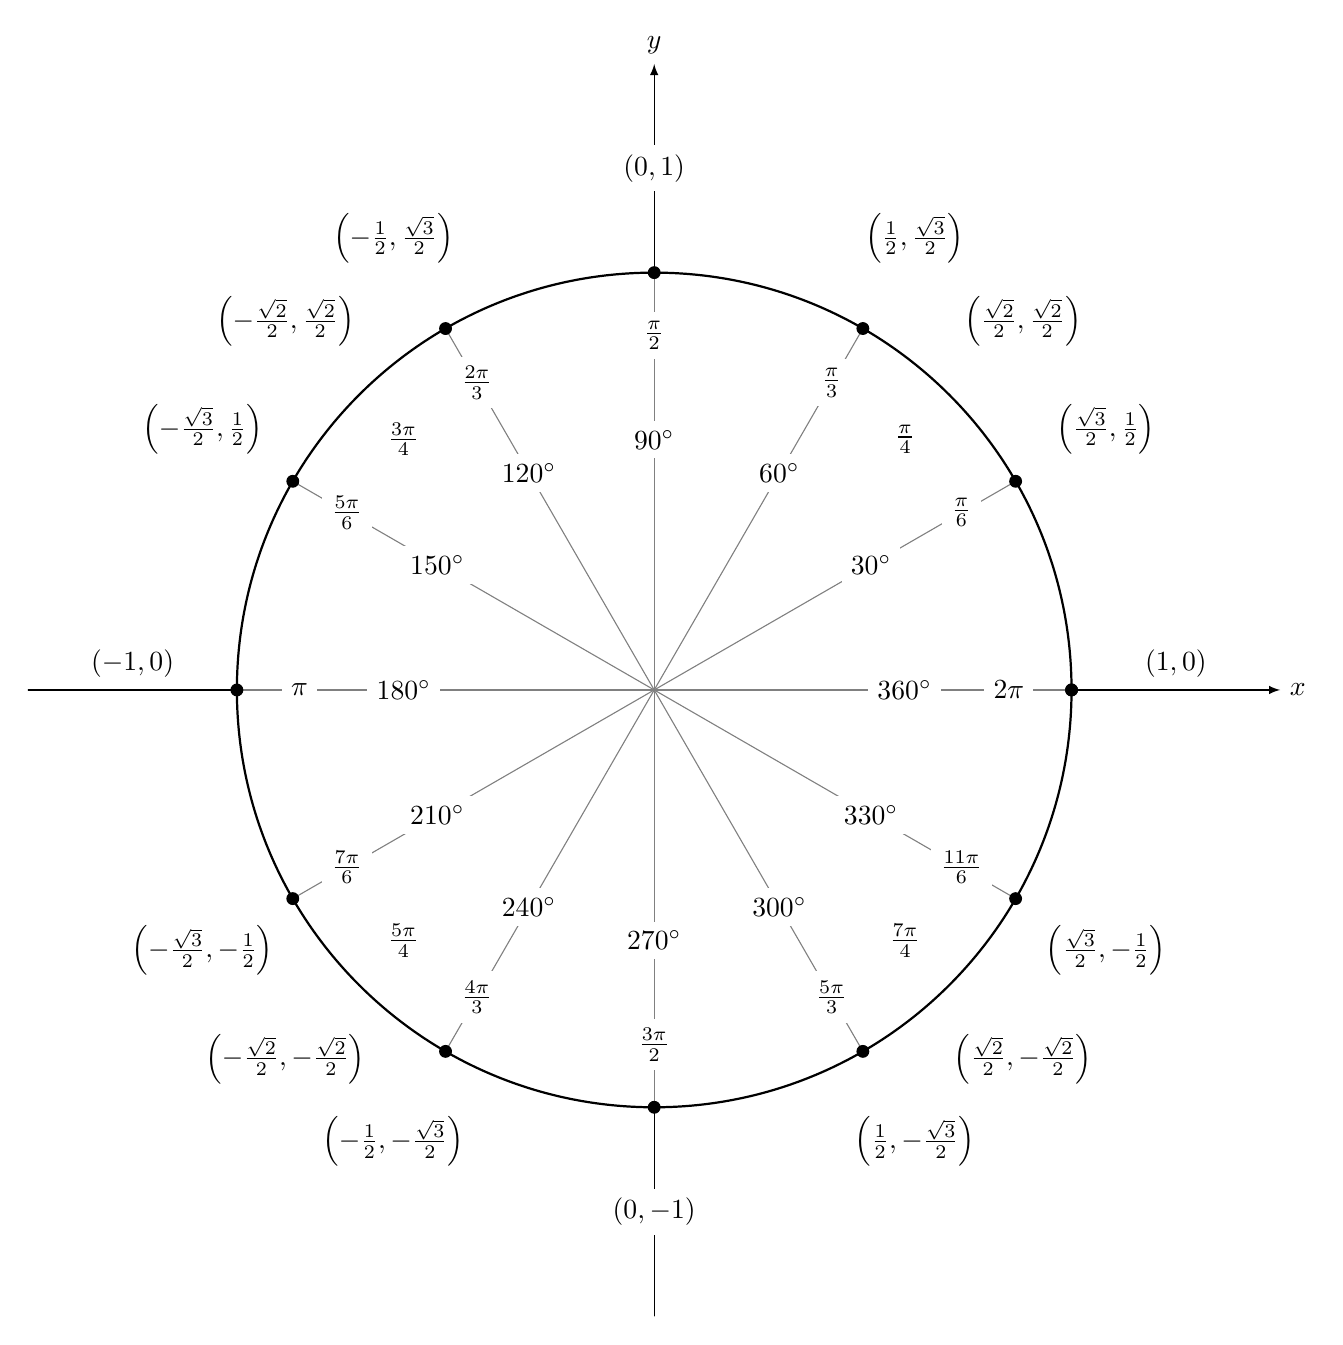
\begin{tikzpicture}[scale=5.3,cap=round,>=latex]
        % draw the coordinates
        \draw[->] (-1.5cm,0cm) -- (1.5cm,0cm) node[right,fill=white] {$x$};
        \draw[->] (0cm,-1.5cm) -- (0cm,1.5cm) node[above,fill=white] {$y$};

        % draw the unit circle
        \draw[thick] (0cm,0cm) circle(1cm);

        \foreach \x in {0,30,...,360} {
                % lines from center to point
                \draw[gray] (0cm,0cm) -- (\x:1cm);
                % dots at each point
                \filldraw[black] (\x:1cm) circle(0.4pt);
                % draw each angle in degrees
                \draw (\x:0.6cm) node[fill=white] {$\x^\circ$};
        }

        % draw each angle in radians
        \foreach \x/\xtext in {
            30/\frac{\pi}{6},
            45/\frac{\pi}{4},
            60/\frac{\pi}{3},
            90/\frac{\pi}{2},
            120/\frac{2\pi}{3},
            135/\frac{3\pi}{4},
            150/\frac{5\pi}{6},
            180/\pi,
            210/\frac{7\pi}{6},
            225/\frac{5\pi}{4},
            240/\frac{4\pi}{3},
            270/\frac{3\pi}{2},
            300/\frac{5\pi}{3},
            315/\frac{7\pi}{4},
            330/\frac{11\pi}{6},
            360/2\pi}
                \draw (\x:0.85cm) node[fill=white] {$\xtext$};

        \foreach \x/\xtext/\y in {
            % the coordinates for the first quadrant
            30/\frac{\sqrt{3}}{2}/\frac{1}{2},
            45/\frac{\sqrt{2}}{2}/\frac{\sqrt{2}}{2},
            60/\frac{1}{2}/\frac{\sqrt{3}}{2},
            % the coordinates for the second quadrant
            150/-\frac{\sqrt{3}}{2}/\frac{1}{2},
            135/-\frac{\sqrt{2}}{2}/\frac{\sqrt{2}}{2},
            120/-\frac{1}{2}/\frac{\sqrt{3}}{2},
            % the coordinates for the third quadrant
            210/-\frac{\sqrt{3}}{2}/-\frac{1}{2},
            225/-\frac{\sqrt{2}}{2}/-\frac{\sqrt{2}}{2},
            240/-\frac{1}{2}/-\frac{\sqrt{3}}{2},
            % the coordinates for the fourth quadrant
            330/\frac{\sqrt{3}}{2}/-\frac{1}{2},
            315/\frac{\sqrt{2}}{2}/-\frac{\sqrt{2}}{2},
            300/\frac{1}{2}/-\frac{\sqrt{3}}{2}}
                \draw (\x:1.25cm) node[fill=white] {$\left(\xtext,\y\right)$};

        % draw the horizontal and vertical coordinates
        % the placement is better this way
        \draw (-1.25cm,0cm) node[above=1pt] {$(-1,0)$}
              (1.25cm,0cm)  node[above=1pt] {$(1,0)$}
              (0cm,-1.25cm) node[fill=white] {$(0,-1)$}
              (0cm,1.25cm)  node[fill=white] {$(0,1)$};
    \end{tikzpicture}
  \end{image}













\begin{example}



Analyze $f(t) = 3 \sin(2t - \pi) - 2$



\begin{explanation}


$\blacktriangleright$ \textbf{One period} \\


Start:  $2t - \pi = 0$, which occurs at $t = \frac{\pi}{2}$where $f = 3 \cdot 0 - 2 = -2$  \\


Finish:  $2t - \pi = 2 \pi$, which occurs at $t = \frac{3 \pi}{2}$, where $f = 3 \cdot 0 - 2 = -2$ \\


Period = $\frac{3 \pi}{2} - \frac{\pi}{2} = \pi$


Halfway between $\frac{\pi}{2}$ and $\frac{3\pi}{2}$ is $\pi$.  \\


$\sin(2t - \pi)$ equals $0$ at $\pi$, where $f = 3 \cdot 0 - 2 = -2$.


A quarter of the way from Start to Finish is $\frac{3 \pi}{4}$, where $f = 3 \cdot 1 - 2 = 1$


The three-quarter mark is $\frac{5 \pi}{4}$, where $f = 3 \cdot -1 - 2 = -5$





\begin{image}
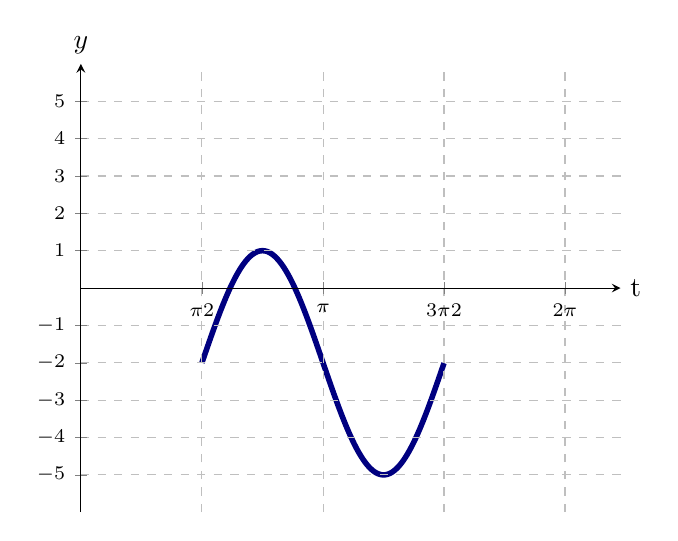
\begin{tikzpicture}
  \begin{axis}[
            domain=0:7, ymax=6, xmax=7, ymin=-6, xmin=0,
            axis lines =center, xlabel={t}, ylabel={$y$}, grid = major, grid style={dashed},
            ytick={-5,-4,-3,-2,-1,0,1,2,3,4,5},
            xtick={0, 1.57, 3.142, 4.71, 6.28},
            xticklabels={$0$, $\tfrac{\pi}{2}$, $\pi$, $\tfrac{3\pi}{2}$, $2\pi$},
            yticklabels={$-5$,$-4$,$-3$,$-2$,$-1$,$0$,$1$,$2$,$3$,$4$,$5$}, 
            ticklabel style={font=\scriptsize},
            every axis y label/.style={at=(current axis.above origin),anchor=south},
            every axis x label/.style={at=(current axis.right of origin),anchor=west},
            axis on top
          ]
          

            \addplot [line width=2, penColor, smooth,samples=300,domain=(1.57:4.71)] {3*sin(deg(2*x-3.14))-2};
            %\addplot [line width=2, penColor2, smooth,samples=300,domain=(-10:10),<->] {cos(deg(x)};


            %\node[penColor] at (axis cs:3.5,1.1) [anchor=north] {$\sin(\theta)$};
            %\node[penColor2] at (axis cs:1.4,1.3) [anchor=north] {$\cos(\theta)$};



  \end{axis}
\end{tikzpicture}
\end{image}



$\blacktriangleright$ \textbf{Then, extend periodically} 








\begin{image}
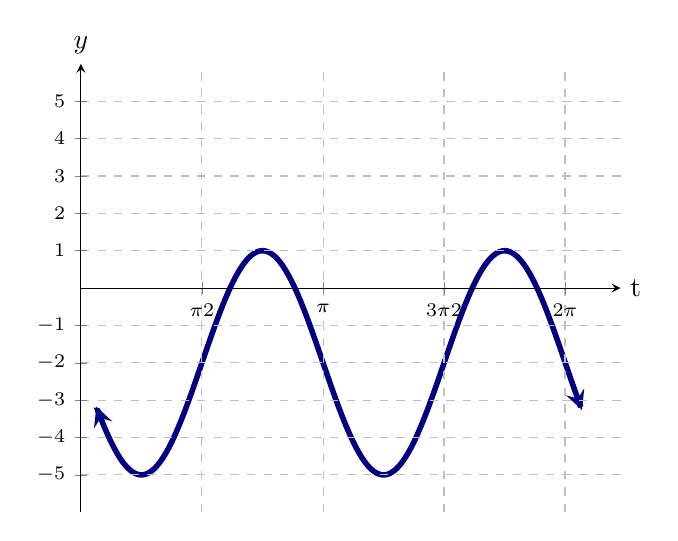
\begin{tikzpicture}
  \begin{axis}[
            domain=0:7, ymax=6, xmax=7, ymin=-6, xmin=0,
            axis lines =center, xlabel={t}, ylabel={$y$}, grid = major, grid style={dashed},
            ytick={-5,-4,-3,-2,-1,0,1,2,3,4,5},
            xtick={0, 1.57, 3.142, 4.71, 6.28},
            xticklabels={$0$, $\tfrac{\pi}{2}$, $\pi$, $\tfrac{3\pi}{2}$, $2\pi$},
            yticklabels={$-5$,$-4$,$-3$,$-2$,$-1$,$0$,$1$,$2$,$3$,$4$,$5$}, 
            ticklabel style={font=\scriptsize},
            every axis y label/.style={at=(current axis.above origin),anchor=south},
            every axis x label/.style={at=(current axis.right of origin),anchor=west},
            axis on top
          ]
          

            \addplot [line width=2, penColor, smooth,samples=300,domain=(0.2:6.5),<->] {3*sin(deg(2*x-3.14)) -2};
            %\addplot [line width=2, penColor2, smooth,samples=300,domain=(-10:10),<->] {cos(deg(x)};


            %\node[penColor] at (axis cs:3.5,1.1) [anchor=north] {$\sin(\theta)$};
            %\node[penColor2] at (axis cs:1.4,1.3) [anchor=north] {$\cos(\theta)$};



  \end{axis}
\end{tikzpicture}
\end{image}




We can calculate some additional exact values at the easy angles. \\



Our principle interval was $\left[ \frac{\pi}{2}, \frac{3\pi}{2}   \right]$, which has a length of $\pi$. \\





$\blacktriangleright$ $30^{\circ} = \frac{\pi}{6}$ is $\frac{1}{12}$ of the normal basic interval $[0, 2\pi]$.  \\


$\frac{1}{12}$ of our period here would be $\frac{1}{12} \cdot \pi = \frac{\pi}{12}$.

Therefore, if we move $\frac{\pi}{12}$ from $\frac{\pi}{2}$, then we should be at the angle where we normally get $\sin(\frac{\pi}{6}) = \frac{1}{2}$.


$\frac{\pi}{2} + \frac{\pi}{12}  = \frac{7\pi}{12}$.

Let's evaluate $f\left( \frac{7\pi}{12} \right)$ and see if we get $\frac{\pi}{6}$ inside the sine function.

\[
f\left( \frac{7\pi}{12} \right) = 3 \sin\left(2 \left(\frac{7\pi}{12} \right) - \pi \right) - 2 = 3 \sin\left( \frac{2\pi}{12} \right) - 2  = 3 \sin\left( \frac{\pi}{6} \right) - 2 = 3 \cdot \frac{1}{2} - 2 = -\frac{1}{2}
\]






\begin{image}
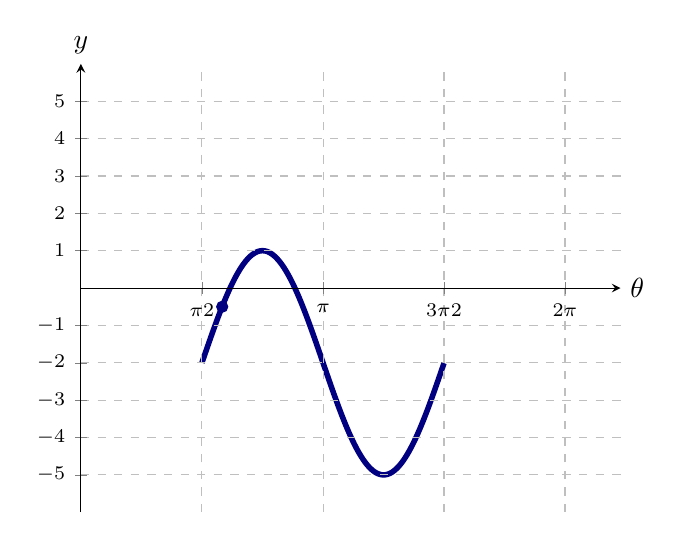
\begin{tikzpicture}
  \begin{axis}[
            domain=0:7, ymax=6, xmax=7, ymin=-6, xmin=0,
            axis lines =center, xlabel={$\theta$}, ylabel={$y$}, grid = major, grid style={dashed},
            ytick={-5,-4,-3,-2,-1,0,1,2,3,4,5},
            xtick={0, 1.57, 3.142, 4.71, 6.28},
            xticklabels={$0$, $\tfrac{\pi}{2}$, $\pi$, $\tfrac{3\pi}{2}$, $2\pi$},
            yticklabels={$-5$,$-4$,$-3$,$-2$,$-1$,$0$,$1$,$2$,$3$,$4$,$5$}, 
            ticklabel style={font=\scriptsize},
            every axis y label/.style={at=(current axis.above origin),anchor=south},
            every axis x label/.style={at=(current axis.right of origin),anchor=west},
            axis on top
          ]
          

            \addplot [line width=2, penColor, smooth,samples=300,domain=(1.57:4.71)] {3*sin(deg(2*x-3.14))-2};
            %\addplot [line width=2, penColor2, smooth,samples=300,domain=(-10:10),<->] {cos(deg(x)};


            %\node[penColor] at (axis cs:3.5,1.1) [anchor=north] {$\sin(\theta)$};
            %\node[penColor2] at (axis cs:1.4,1.3) [anchor=north] {$\cos(\theta)$};

            \addplot[color=penColor,fill=penColor,only marks,mark=*] coordinates{(1.833,-0.5)};



  \end{axis}
\end{tikzpicture}
\end{image}









$\blacktriangleright$ $60^{\circ} = \frac{\pi}{3}$ is $\frac{1}{6}$ of the normal basic interval $[0, 2\pi]$.  \\

$\frac{1}{6}$ of our period here would be $\frac{1}{6} \cdot \pi = \frac{\pi}{6}$.

Therefore, if we move $\frac{\pi}{6}$ from $\frac{\pi}{2}$, then we should be at the angle where we get $\sin(\frac{\pi}{3}) = \frac{\sqrt{3}}{2}$.


$\frac{\pi}{2} + \frac{\pi}{6} = \frac{4\pi}{6} =  \frac{2\pi}{3}$.

Let's evaluate $f\left( \frac{2\pi}{3} \right)$ and see if we get $\frac{\pi}{3}$ inside the sine. \\

\[
f\left( \frac{2\pi}{3} \right) = 3 \sin\left(2 \left(\frac{2\pi}{3} \right) - \pi \right) - 2 = 3 \sin\left( \frac{\pi}{3} \right) - 2  =  3 \cdot \frac{\sqrt{3}}{2} - 2 = \frac{3\sqrt{3}-4}{2} \approx 0.5980762114
\]










\begin{image}
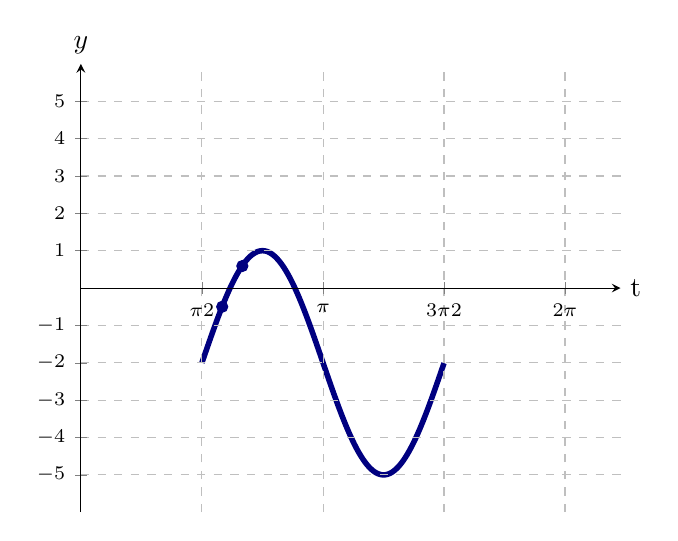
\begin{tikzpicture}
  \begin{axis}[
            domain=0:7, ymax=6, xmax=7, ymin=-6, xmin=0,
            axis lines =center, xlabel={t}, ylabel={$y$}, grid = major, grid style={dashed},
            ytick={-5,-4,-3,-2,-1,0,1,2,3,4,5},
            xtick={0, 1.57, 3.142, 4.71, 6.28},
            xticklabels={$0$, $\tfrac{\pi}{2}$, $\pi$, $\tfrac{3\pi}{2}$, $2\pi$},
            yticklabels={$-5$,$-4$,$-3$,$-2$,$-1$,$0$,$1$,$2$,$3$,$4$,$5$}, 
            ticklabel style={font=\scriptsize},
            every axis y label/.style={at=(current axis.above origin),anchor=south},
            every axis x label/.style={at=(current axis.right of origin),anchor=west},
            axis on top
          ]
          

            \addplot [line width=2, penColor, smooth,samples=300,domain=(1.57:4.71)] {3*sin(deg(2*x-3.14))-2};
            %\addplot [line width=2, penColor2, smooth,samples=300,domain=(-10:10),<->] {cos(deg(x)};


            %\node[penColor] at (axis cs:3.5,1.1) [anchor=north] {$\sin(\theta)$};
            %\node[penColor2] at (axis cs:1.4,1.3) [anchor=north] {$\cos(\theta)$};

            \addplot[color=penColor,fill=penColor,only marks,mark=*] coordinates{(1.833,-0.5)};
            \addplot[color=penColor,fill=penColor,only marks,mark=*] coordinates{(2.094,0.59)};



  \end{axis}
\end{tikzpicture}
\end{image}







\end{explanation}


\end{example}






\begin{summary} Sine and Cosine \\


Sine and Cosine are basically shifts of each other.  They follow the same periodic patterns. \\

They both oscillate between $-1$ and $1$, which makes their range $[-1,1]$. \\

They both have their maximum value of $1$ and their minimum value of $-1$ at the top, bottom, or sides of the unit circle. \\

When one has maximum or minimum, the other has a zero. \\

\end{summary}


When we analyze sine and cosine functions, we usually start by locating when the inside is $0$, $\frac{\pi}{2}$, $\pi$, $\frac{3\pi}{2}$, or $2\pi$.  This tells us when the function is experiencing a maximum, minimum, or zero.

Then we move to the easy angles ($\frac{\pi}{6}$, $\frac{\pi}{4}$, and $\frac{\pi}{3}$) to round out the shape. \\





\textbf{\textcolor{red!80!black}{$\blacktriangleright$}} This is how we analyze compositions involving sine and cosine.







\end{document}
